\title{A Very Simple \LaTeXe{} Template}
\author{
        Vitaly Surazhsky \\
                Department of Computer Science\\
        Technion---Israel Institute of Technology\\
        Technion City, Haifa 32000, \underline{Israel}
            \and
        Yossi Gil\\
        Department of Computer Science\\
        Technion---Israel Institute of Technology\\
        Technion City, Haifa 32000, \underline{Israel}
}
\date{\today}

\documentclass[14pt]{article}
\usepackage[a4paper, total={6in, 8in}]{geometry}
\usepackage{graphicx}
\usepackage{verbatim} 
\renewcommand{\baselinestretch}{1.3}

\begin{document}
\maketitle

\begin{abstract}
This is the paper's abstract \ldots
\end{abstract}

\section{Introduction}
Correctness of computer systems is important in our software dependent society. We depend more and more on this modern computer systems. Such systems consist of complex hardware and software components. So correctness of both hardware and software is important. However, it is much harder to ensure the correctness of the software part of these systems. As the complexity of the software parts are getting more complex than that of the underlying hardware.  And manual inspection of complex software is error-prone and costly.  Numerous formal tools to find functional design bugs in hardware are available and in wide-spread use.  In contrast, the market for software verification tools is still in its infancy. A lot of research in this field is going on. We need highly automated method that provides rigorous guarantee of quality. These methods should be scalable enough to match the enormous complexity of software systems. Bounded model checking (BMC) of programs is one of such methods used for software verification. In this paper we will explore LLBMC, an implementation of the idea of  Bounded model checking.

\paragraph{Outline}
The remainder of this article is organized as follows.
Section~\ref{previous work} gives account of previous work.
Our new and exciting results are described in Section~\ref{results}.
Finally, Section~\ref{conclusions} gives the conclusions.

\section{Verification problem}\label{verification problem}
In industry we see the use of testing to ensure software quality and even to find bugs. However such quality guarantees do not reflect to "correctness" of  the system. As we know that ensuring the absence of all errors in a design is usually too expensive. So all testing based approaches e.g. random testing and automated test-case generation are incomplete.  The other approach depends on the fact that systems can be viewed as mathematical objects with well-specified behaviour. Or we can specify the system (intended behaviour) using mathematical logic. Then one can reason about whether the system meets its specification or not. This field of study has been active and it is often referred to as formal methods. The \textit{verification problem} is: Given program \textit{M} and specification \textit{h} determine whether or not the behaviour of \textit{M} meets the specification \textit{h}. The specification is formulated in mathematical logic. The model checking problem is an instance of the verification problem. Model checking provides an automated method for verifying finite state systems and checks it for certain properties. The method is algorithmic and often efficient because the system is finite state. If the check fails, that means the design has a bug. And, most of the time, the model checkers generate a counterexample how the bug is produced so the developer can easily figure out what is the mistake.

\section{Bounded Model Checking}\label{bounded model checking}

Model checking is a method for formally verifying finite-state systems. Specifications about the system are expressed as temporal logic formulas, and efficient symbolic algorithms are used to traverse the model defined by the system and check if the specification holds or not. Extremely large state-spaces can often be traversed in minutes.
					
Bounded Model Checking is first proposed by Biere et. al. in 1999 ~\cite{1}. It doesn't reduce the complexity of model checking however, it can solve many cases which cannot be solved by BDD (binary decision diagram) based techniques. However, BMC has the disadvantage of not being able to prove the program is valid because of its bounded state structure.
					
Idea of BMC is searching for a counterexample in the given problem until an execution length n. The BMC problem can be efficiently reduced to a propositional satisfiability problem and can be solved by SAT solvers. Modern SAT solvers can handle propositional satisfiability problems with 6-7 digit variables and sometimes more.
					
However, as stated previously, BMC approach is used for finding bugs, not for proving the program is valid because of the execution length. A greater execution length might show bugs which cannot be found for smaller execution lengths.
					
In formally, bounded model checking contains: A transition system, a temporal logic formula and a user supplied bound k. Using these properties, we check if the given formula satisfied in the given bound.
					
In our work, the program flow is described as transition states for the BMC conversion. The easy transform between BMC and SMT formulas is highly beneficial because of the presence of highly optimised SMT solvers.

\section{LLVM}\label{llvm}
LLVM (Low Level Virtual Machine) is a compiler infrastructure; designed for compile-time, link-time, run-time, and "idle-time" optimization of programs written in different various programming languages. Initially designed for C and C++, LLVM now supports a lot of different languages like ActionScript, Ada, D, Fortran, GLSL, Haskell, Java, Julia, Objective-C, Python, Ruby, Rust, Scala.
					
LLVM supports a language-independent instruction set and type system. [3] Each instruction is in static single assignment form (SSA), meaning that each is assigned only once and cannot be assigned again. This helps simplify the analysis of dependencies among variables. LLVM allows code to be compiled statically, as it is under the traditional GCC system, or left for late-compiling from the IF to machine code in a just-in-time compiler (JIT) fashion similar to Java. The type system consists of primitive types such as integers or floats and five other derived types: Arrays, vectors, functions, structures and pointers. A type construct is represented by combining these given types in LLVM. For example, a class in C++ can be represented by a combination of structures, functions and arrays of function pointers.
					
LLVM is used in many areas because of its optimization supporting and competitive performance results. For example, Apple uses LLVM in its Xcode and Cocoa frameworks [10].
					
LLVM adapted SSA (Static Single Assignment) form. This provides serious advantages for formal conversions. The instruction set composed three address code instructions. Also, the LLVM instructions in Linux can generate CFG (control flow graphs) of the threads and the program which helps our conversion. Because LLVM-IR is represented in a similar format with 3 address assembly instructions, the adaptation period for unfamiliar users should not take very long, considering the developer already had some experience with Assembly. 

\section{SMT-LIB}\label{SMT-LIB}
Satisfiability Modulo Theories (SMT) have the aim of testing logical formulas for if they are satisfiable or not, using one or more theories. An SMT instance is a formula in first order logic, where some function and predicate symbols might have additional interpretations, and SMT is the problem of determining if such a formula is satisfiable. In other words, imagine an instance of the Boolean satisfiability problem (SAT) in which some of the binary variables are replaced by predicates over a suitable set of non-binary variables. A predicate is basically a binary-valued function of non-binary variables [5] [8].
					
One of the earlier attempts for solving SMT instances was translating them to SAT instances (e.g., a 32-bit integer variable would be encoded by 32 bit variables with appropriate weights) and passing this formula to a Boolean SAT solver because of the existing optimized SAT solvers. This approach, which is referred to as the eager approach, has its merits: by preprocessing the SMT formula into an equivalent Boolean SAT formula we can use existing Boolean SAT solvers "as-is" and leverage their performance and capacity improvements over time. However, the loss of the high-level semantics of the underlying theories means that the Boolean SAT solver has to work a lot harder than necessary to discover "obvious" facts (such as x + y = y + x for integer addition.) This observation led to the development of a number of SMT solvers that tightly integrate the Boolean reasoning of a DPLL-style search with theory specific solvers (T-solvers) that handle conjunctions (ANDs) of predicates from a given theory. This approach is referred to as the lazy approach [5] [7]. 

SMT-LIB is a functional language similar to LISP. SMT-LIB was created with the expectation that the availability of common standards and a library of benchmarks would greatly facilitate the evaluation and the comparison of SMT systems, and advance the state of the art in the field in the same way as, for instance, the TPTP library has done for theorem proving, or the SATLIB library has done initially for SAT [6]. 

Our approach can be summarized as follows: First, converting the multi-threaded code (we are working on C programs at the moment) to LLVM IR format with certain optimizations. Then converting this intermediate code to SMT-LIB format and creating a model of the program in a valid SMT formula. Lastly, giving this model to a SMT checker (MathSAT5) to find if the program has a bug for the given execution length. 


\section{What is LLMBC?}\label{overview-LLMBC}
LLBMC (the low-level bounded model checker) is a static software analysis and verification tool for finding bugs in C (and, to some extent, in C++) programs. It is based on the technique of Bounded Model Checking. It is mainly intended for checking low-level system code.  It takes sequential C/C++ programs and finds bugs and runtime errors. It can help 
software engineers to improve the quality of software and obtain stable and secure programs and reduce the time and effort needed for software testing. 

LLBMC is fully automatic and requires minimal preparation efforts and user interaction. it models memory accesses (heap, stack, global variables) with high precision and is thus able to find hard-to-detect memory access errors like heap or stack buffer overflows. LLBMC can also uncover errors due to uninitialized variables or other sources of non-deterministic behaviours e.g.  
\textit{integer overflow}, 
\textit{division by zero},
\textit{invalid bit shift},
\textit{illegal memory access (array index out of bound, illegal pointer access, etc.)},
\textit{invalid free},
\textit{double free},
\textit{user-customizable checks}.
We will explain more on these built-in-checks in subsequent sections. 

The main limitation of LLBMC is its incompleteness. As it is just an implementation of the idea of BMC, its makes it incomplete due to incompleteness of the bounded analysis. Other limitations are it's high program-dependency and scalability. 

\section{Why Low-Level}\label{Low-Level}
We know that LLBMC takes a program in C code and finally reports bugs. However it does not directly work on source code. Applying BMC for verifying C programs is very hard and comes with many obstacles that have to be tackled. One of the most important differences is that the syntax (and thus semantics) of a high level programming language like C is much more complicated than a hardware description. Issues like memory allocation, (function) pointers, complex data structures, and function calls have to be managed. Further more going from C to C++ introduces more complex issues. Thats why instead of exploring the source code directly, LLBMC makes use of existing compiler technology and performs the analysis on an assembler-like compiler intermediate language. Such an intermediate language offers a much simpler syntax (and semantics), and thus eases a logical encoding of the verification problem considerably. We will describe more on how LLBMC uses LLVM-IR for the analysis. We can summarise the advantages of this approach as,
\begin{itemize}
   \item The IR has much simpler syntax and semantics than C/C++. This makes it relatively easy to support (nearly) all language features.
     \item The program that is analysed is much closer to the program that is actually executed on the hardware since semantic ambiguities are resolved by the compiler. Furthermore, it becomes possible to analyze programs at various optimisation levels offered by the compiler.
  \item It becomes possible to analyse programs in any language for which a compiler frontend that produces the IR is available.
  
\end{itemize}

\section{Software Bounded Model Checking}\label{Software Bounded Model Checking}
Here we briefly describe the main ideas of bounded model checking for software especially for programs written in C/C++. Generally programs are composed of data structures such as linked lists or trees. The unbounded nature of such data structures may give rise to infinite program runs. Which is very common in all kind of systems e.g.  in reactive or interactive systems.  Property checking of such programs is in general undecidable.  Here bounded model checking provides a solution. BMC limits such program runs to finite ones, thereby achieving decidability. The bound is imposed by restricting the number of nested function calls and loop iterations that are considered. BMC performs function inlining and loop unrolling (up to these bounds), resulting in one large function that is then subject to further analysis. Since the analysis is done on the finite run of the program, it  can only look for bugs up to specific depth. This is good enough for many applications e.g. embedded systems. 

Here we will see an example of loop unrolling for a simple program. We assume that properties for the program are given by assertions from  the user. And we need to verify that these properties holds for the program where the loop iteration is bounded by number k. The states that the program can reach within this bound are represented symbolically by a formula, together with the negation of the given condition. Then this combined formula is feed to SAT solver. If the formula is satisfiable, then there exists a path in the program that violates the property.

\begin{figure}[htb!]
  \begin{centering}
    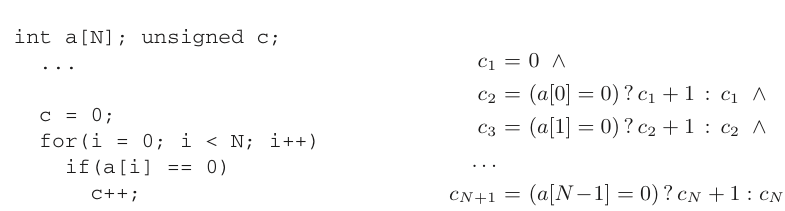
\includegraphics[width=\textwidth]{figures/bmc-example-1}\par
  \end{centering}
  \caption{A simple dummy picture to demonstrate how
           to include graphics into your report.}
  \label{fig:mesh1}
\end{figure}



Consider the program in the left part of figure \ref{fig:mesh1}. The number of paths through this program is exponential in \(N\), as each of the \(a[i]\) elements can be either zero or nonzero. Despite the exponential number of paths through the program, its states can be encoded with a formula of size linear in \(N\), as demonstrated in the right part of the figure. This formula encodes the states of the original program on its left, using the static-single-assignment (SSA) form. 		 	 	 		

\begin{figure}[htb!]
  \begin{centering}
    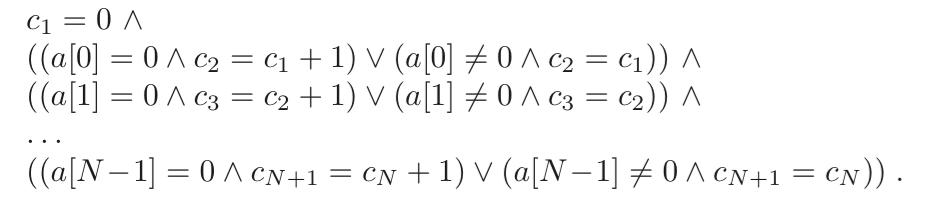
\includegraphics[width=0.80\textwidth]{figures/bmc-example-2}\par
  \end{centering}
  \caption{formula after all the rewrite is donw.}
  \label{fig:mesh2}
\end{figure}

The ternary operator \(c?x:y\) in the equation on the right of figure \ref{fig:mesh1} can be rewritten using a disjunction, as shown in figure \ref{fig:mesh2}. After the rewrite we have the formula in DNF. Now to verify that some assertion provided by user holds at a specific, we add a constraint corresponding to the negation of this assertion. For example, to prove that at the end of the program \(c \leq N\) , we need to conjoin formula with \((c_{N+1}>N)\). Now we can test this combined formula for satisfiability. 

In this example we have shown how the idea works on the source code level. We will see how llbmc models this idea of Bounded Model Checking. Properties of a program are typically expressed  as pre-condition( \(assume\) ) or post-conditions( \(assert\) ). Where assume states a pre-condition that is assumed to hold at its location and assert states a post-condition that is to be checked at its location. The program  \(Prog\)  is correct if
\[Prog \wedge \bigwedge assume \Rightarrow  \bigwedge assert\]
is valid. This check is decided using SAT or SMT solver. 


\section{LLBMC approach}\label{lbmc approach}
Here we will explain how llbmc model the verification problem.  Figure \ref{fig:llbmc_overview} shows the overall structure of llbmc approach.  
\begin{figure}[htb!]
  \begin{centering}
    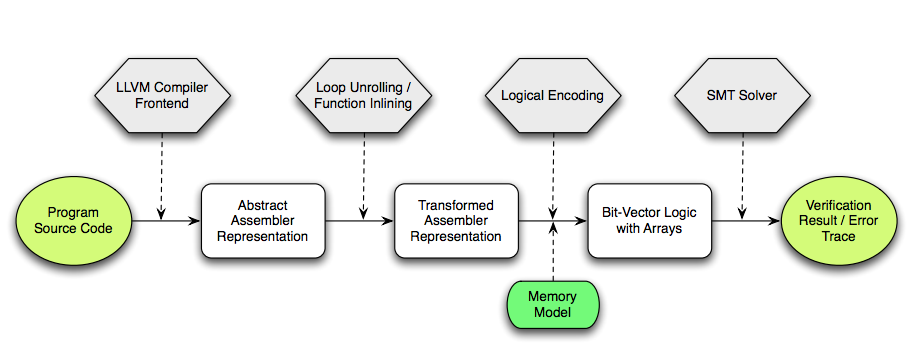
\includegraphics[scale=0.5]{figures/llbmc_overview}\par
  \end{centering}
  \caption{ Overview of llbmc approach. Image is taken from \cite{llbmc2}.}
  \label{fig:llbmc_overview}
\end{figure}



\subsubsection{LLVM Intermediate Representation}
llbmc makes extensive use of llvm compiler framework. it uses the llvm compiler front end to get the program in LLVM abstract assembler from program source code. Since programs in LLVM assembler are already in \textit{static single assignment (SSA)} form, assignments to scalar variables are treated as logical equivalences. However, other LLVM instructions need to be handled. 
In the context of llbmc the following LLVM instructions are important and we will show how each of these instructions are translated into the logic of bit-vectors and arrays. 
\begin{itemize}
  \item \textit{Three-address-code (TAC)} instructions working on registers or constants.
  \item \textit{Memory access and allocation} instructions, namely \texttt{load, store, malloc}, and \texttt{free}.
  \item \textit{Address calculations} using \texttt{getelementptr}.
  \item \textit{Branch and phi} instructions.
\end{itemize}

\subsubsection{Function inlining and loop unrolling} 
Before starting the process of logical encoding, the program must be transformed (from llvm-ir to llvm-ir) so that it finishes with a finite run. llbmc uses code provided by the LLVM libraries to do this function inlining and loop unrolling. The control flow graph get simplified after this transformation. After the loop unrolling the graph becomes directed acyclic graph. LLBMC uses the debug information generated by LLVM to report error trace back to user.

\subsubsection{Logical Encoding}\label{Logical Encoding}
After function inlining and loop unrolling, llvm program is ready to be encoded into the logic of bit-vectors and arrays. The complete logical encoding is done in several stages. First the initial SMT encoding is done. Basic blocks are ( and their execution conditions) still present in this initial SMT encoding.  We will briefly explain how llbmc handles few important llvm instructions.
\par \textit{Handling of assignments:} Since llvm assembly is in SSA form, assignments are treated as equalities.
\par \textit{Handling of Three-address-code (TAC) Instructions:}  These instructions (like, e.g.,add, cmp, mul, sign or zero extension) are supported by SMT solvers. So their translation is straightforward.
\par \textit{Handling of phi Instructions:} Every phi instruction can be translated into a sequence of ITE (if-then-else) operators, which are also supported by SMT solvers. More on this can be found in \cite{llbmc2}.
\par \textit{Handling of The }\texttt{getelementptr}  \textit{Instruction:} Every \texttt{getelementptr}  instruction is simply transformed into a linear equation as shown bellow.
\[q = \texttt{getelementptr} \  p, o_1, \cdots , o_k \   \rightarrow  \   q = p + o_1 . s_1 + \cdots  + o_k .s_k \] 

where \(p\), \(q\) are pointers and the \(o_i\)'s are offsets and the constant multiplicands \(s_i\) can be computed easily based on the
data type definitions and the type of pointer \(p\).

\par \textit{Elimination of Branches:} At this point memory access instructions are need to handled. LLBMC models the memory as an array of bytes. The idea here is to translate llvm memory instructions e.g.,  \texttt{malloc, store, free}. LLBMC propose SSA form for the memory by introducing an explicit memory state and instructions \texttt{read, write, malloc, free}. Memory is accessed using \texttt{read} instructions and Memory is changed using \texttt{write, malloc and free} instructions. LLBMC introduce \texttt{phi} -instructions for memory states, which serve the same purpose as ordinary \texttt{phi} instructions for scalar values. At this point the conversion of memory to SSA form and  encoding of \texttt{phi} instructions branches are no longer needed.

\par \textit{Encoding Memory Constraints:} LLBMC provides following built-in memory checks. 
\begin{itemize}
  \item \textit{Valid read/writes } (i.e. only to allocated memory).
  \item \textit{Valid frees} (i.e. \texttt{free} is only called for a block of allocated memory).
  \item \textit{No double frees} (i.e. no memory block is  \texttt{free}'d twice).
  \item \textit{No memory leaks} (i.e. all allocated heap memory is de-allocated when the program ends).
\end{itemize}
llbmc introduces few predicates ( and needed formulas) on the memory state: 
  \texttt{valid\_mem\_access},
  \texttt{deallocated},
  \texttt{non\_overlap},
  \texttt{malloc\_assumption},
  \texttt{valid\_free},
  \texttt{no\_memory\_leaks}. The definitions of these memory consistency predicates can be found in \cite{llbmc2}. Here we will see how these predicates helps to generate memory consistency constraints for \textit{valid read/writes } checks. The idea here is to add appropriate guards before/after the memory access instructions. These guards are taken from the defined memory consistency predicates. For the \textit{Valid read/writes } check, llbmc first add an \texttt{assume(malloc\_assumption( }\(m', p, s\) \texttt{)} statement after each \(m' = \texttt{malloc}(m, p, s)\) instruction. Then llbmc add \(\texttt{assert(valid\_mem\_access(}m, p, s\texttt{))}\) before each \( m' = \texttt{write}(m, p, x)\) and \( x = \texttt{read}(m, p)\) instruction, where  \(s\) is the size in bytes of the data to be read or written. Having processed all \texttt{malloc}s, \texttt{read}s and \texttt{write}s, the \texttt{malloc} and \texttt{free} instructions can be removed. After this stage of transformation, llbmc uses the defined formulas to translate the predicates into the logic of bit-vectors and arrays.
  
 \par \textit{Adding other checks to the ILR formula:} This initial ILR formula is annotated with LLBMC's other built-in checks. Most of these checks are supported by a predicate that is part of ILR. Then, an instruction that can possibly overflow is guarded by assertion that no overflow occurs and so on. 
 
 \par \textit{Simplification of the ILR formula:} LLBMC uses term rewriting in order to simplify the ILR formula before passing it to an SMT solver. LLBMC implements  approximately 150 (conditional) rewrite rules \cite{llbmc0}. As all ILR's predicates for built-in checks are not supported by SMT-solver, those predicates are expanded. e.g. checks for logic and arithmetic shift which can easily be encoded in bit-vector logic. After expanding the predicates for the built-in checks and rewrite-based simplifications of the formula, it is ready to be passed to the SMT solver.
  
  
  \subsubsection{Counterexample generation}\label{Counterexample generation} The simplified ILR formula is then passed to an SMT solver. If the formula is satisfiable, any satisfying assignment corresponds to a bug in the program. By mapping ILR variables to the corresponding instructions in the LLVM-IR program and simulating execution with these values, a trace of the LLVM-IR program that exhibits the bug can be obtained. 
  
  
\section{Evaluation}\label{Evaluation}
LLBMC can be compared with two other BMC tools: the C Bounded Model Checker CBMC  \cite{CBMC} and the Efficient SMT-Based
11Context-Bounded Model Checker ESBMC  \cite{ESBMC}. According to paper \cite{llbmc0},  an empirical evaluation on a large collection of C programs is conducted.  The evaluation has shown that LLBMC compares favourably to CBMC and ESBMC, both in run-time and in number of found bugs. Furthermore, LLBMC has successfully been used on over 50 non-trivial C++ programs. 
  
 \section{Conclusions}\label{conclusions}
We worked hard, and achieved very little.
  
\begin{figure}[htb!]
  \begin{centering}
    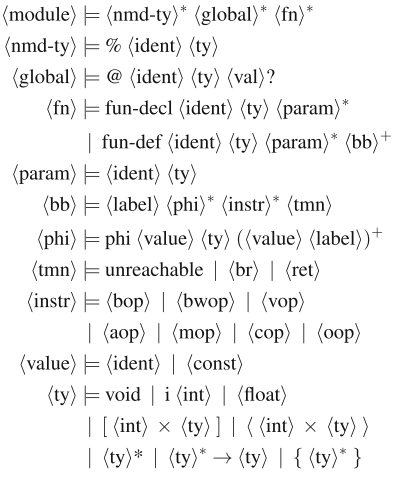
\includegraphics[scale=0.5]{figures/llvm_ir_grammar}\par
  \end{centering}
  \caption{Abstract LLVM IR grammar}
  \label{fig:llvm_ir_grammar}
\end{figure}

\begin{figure}[htb!]
  \begin{centering}
    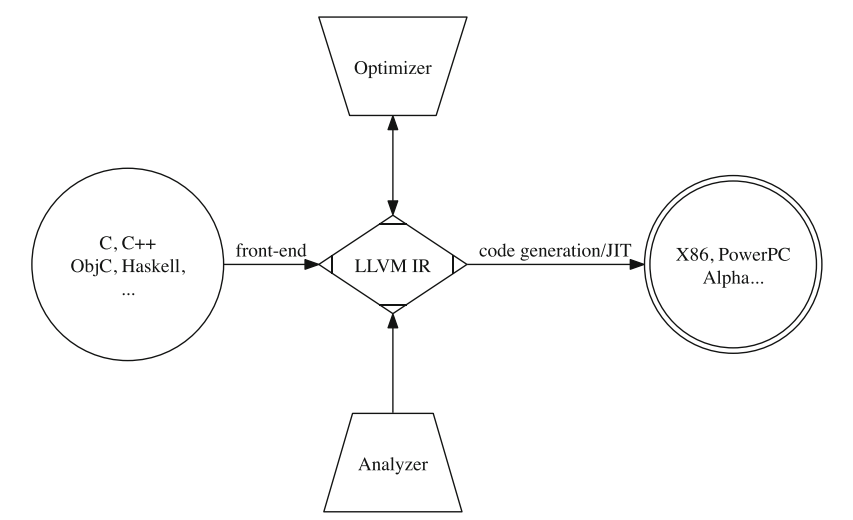
\includegraphics[scale=0.5]{figures/llvm_architecture}\par
  \end{centering}
  \caption{LLVM architecture}
  \label{fig:llvm_architecture}
\end{figure}

\begin{thebibliography}{9}
\bibitem{bmc} 
Edmund Clarke, Armin Biere, Richard Raimi and Yunshan Zhu
\textit{Bounded Model Checking Using Satisfiability Solving}.

\bibitem{1} 
Armin Biere, Alessandro Cimatti, Edmund Clarke, Yunshan Zhu
\textit{Symbolic Model Checking without BDDs}. 

\bibitem{llbmc} 
Stephan Falke, Florian Merz, Carsten Sinz.
\textit{The Bounded Model Checker LLBMC}. 
http://llbmc.org

\bibitem{llbmc2} 
Stephan Falke, Florian Merz and Carsten Sinz.
\textit{A Precise Memory Model for Low-Level Bounded Model Checking}.
http://llbmc.org.

\bibitem{llbmc3} 
Stephan Falke, Florian Merz and Carsten Sinz.
\textit{A Theory of C-Style Memory Allocation}.
\texttt{http://llbmc.org/files/papers/SMT11.pdf}

\bibitem{llbmc0} 
Stephan Falke, Florian Merz and Carsten Sinz.
\textit{LLBMC: Bounded Model Checking of C and C++ Programs Using a Compiler IR*}

\bibitem{ESBMC} 
Lucas Cordeiro, Bernd Fischer, Joao Marques-Silva 
\textit{SMT-based bounded model checking for embedded ANSI-C software}

\bibitem{CBMC} 
Edmund Clarke, Daniel Kroening, and Flavio Lerda
\textit{A tool for checking ANSI-C programs}

\end{thebibliography}

\end{document}
This is never printed
